\section{Experimental Results}
\label{sec:experimentation}

In this section, we present the experiments on text outlier analysis
using matrix factorization. We used both real and synthetic data
sets to test our algorithm. The  real data sets correspond to the
well known {\em RCV20}, {\em Reuters} and {\em Wiki People} data, whereas the
synthetic data set was created using a well known market basket
generator described later.  It should be pointed out that these data
sets were not originally designed for outlier analysis, and they
have no ground truth information available.  Therefore, some
additional pre-processing needed to be applied to the real data
sets, in order to isolate ground truth classes, and use them
effectively for the outlier analysis problem. In this section, we
will describe the data sets, their preparation, the performance
criteria and the results obtained by our algorithm. At the end of
this section, we will also present a discussion that provides
interesting insights about  the effectiveness of algorithm \algo\ .

\subsection{Data Sets}
The experiments were  conducted with both labelled real  and
synthetic data sets.  These are described below:\\
{\bf\em RCV20 Data Set:}  The {\em RCV20 data set}
\footnote{\url{http://qwone.com/~jason/20Newsgroups/}}
 is a collection of approximately 20,000
newsgroup documents, partitioned (nearly) evenly across 20 different
newsgroups. We took all data points from two randomly chosen
classes, which in this case corresponded to the {\em IBM} and {\em
Mac Hardware} classes. In addition, 50 data points were chosen from
one randomly chosen class, which corresponds to the {\em Windows
Operating System (OS)} class. As it turns out, this is a rather hard
problem for  our algorithm because of some level of relationship
between one of the rare classes and the base data. Specifically,
{\em Windows Operating System} and {\em IBM Hardware} are both
computer related subjects, and the former is often used with the
latter. Therefore, some vocabulary is shared between the regular
class and the rare class, and this makes the detection of outlier
harder. We randomly permuted the position of the outliers and
regular data points. \\
{\bf\em Reuters-21578 Data Set:}  The documents in the {\em
Reuters-21578} collection
\footnote{\url{http://archive.ics.uci.edu/ml/datasets/Reuters-21578+Text+Categorization+Collection}}
 appeared on the {\em Reuters} newswire in 1987. It contains  21578 documents in 135
categories. Every document belongs to one or  more categories.
We selected those documents that belong to only one category.
We chose totally 5768 documents that belong to the category {\em earn} and {\em acq}.
The outliers were 100 documents from category {\em interest}. The vocabulary size
of all the documents from these categories put together were 18933.
We randomly permuted the position of the outliers and
regular data points.
\\
\ramki{{\bf\em Wiki People Dataset:} This is a subset of the dataset
collected by Blasiak et.al., \cite{Blasiak13}. The dataset is
constructed by crawling Wikipedia starting from
\url{http://en.wikipedia.org/wiki/Category:Lists_of_politicians} to
a depth of four. Pages describing people were extracted from the
list of all crawled pages. Text from the body paragraphs of the
pages were extracted, and section headings were used as labels for
blocks of text. Text blocks were assumed  to begin with <p> and end
with </p>. Only text in section headings that occurred 10 times or
more was retained. Words were stemmed, stopwords were removed, and
words of length at least 3 and  at most 15 were considered. The
words need to occur at least 4 times in at least 2 documents to be
considered important enough to be  retained. From the collected
data, the sections {\em Career} and {\em Life} were chosen as
non-outlier and whereas the small section  section {\em Death} was
chosen as outlier. The constructed dataset has a vocabulary size of
18834 and total of 9593 documents.  A total of 100 documents that
belong to section {\em Death} were labeled as outlier. }
 \\
{\bf\em  Market Basket Data Generator:} We also wanted to
understand the performance of our algorithm in some large sparse
matrices that is similar to the bag of words matrix. Towards this end, we used the standard {\em
IBM Synthetic Data Generation Code for Associations and Sequential
Patterns} -- market-basket data generator, that is packaged as part
of {\em Illimine}\footnote{\url{http://illimine.cs.uiuc.edu/}}
software. We set the average length of the transaction to be 300 and
number of different items to be 50,000. Note that this generator
uses a random seed, and by changing the seed, it is possible to
completely change the transaction distribution, even if all other
parameters remain the same. We generated 10,000 data points as a
group of four different  sets of 2500 data points with randomly
chosen  seed values. In addition, the rare class contained 250 data
points from a single seed value.  In addition, we randomly permuted
the positions of the outliers and regular data points in the matrix
representation, to avoid any unforeseen bias in the algorithm.

\subsection{Performance Metrics}
The effectiveness was measured in terms of the ROC curve drawn on
the outlier scores. We use the area under the Receiver Operating
Characteristics(ROC) curve -- the defacto metric for evaluation in
outlier analysis. The idea of this curve is to evaluate a {\em
ranking} of outlier scores, by examining the tradeoff between the
true positives and false positives, as the threshold on the outlier
score is varied in a range. By using different thresholds, it is
possible to obtain a relatively larger or smaller number of true
positives with respect to the false positives.

Let $S(t)$ be the set of outliers determined by using a threshold
$t$ on the outlier scores. In this case,  the {\em True Positive
Rate} is graphed against the {\em False Positive Rate}. The true
positive rate $TPR(t)$ is defined in the same way as the metric of
recall is defined in the IR literature. The false positive rate
$FPR(t)$ is the percentage of the falsely reported positives out of
the ground-truth negatives. Therefore, for a data set $D$ with
ground truth positives $G$, these definitions are as follows:
\begin{equation*}
TPR(t)= Recall(t)= 100* \frac{ |S(t) \cap G|}{|G|}
\end{equation*}
\begin{equation*}
FPR(t) =100 * \frac{|S(t) -G|}{|D - G|}
\end{equation*}
 Note that the end points of the ROC curve are
always at $(0, 0)$ and $(100, 100)$, and a random method is expected
to exhibit performance along the diagonal line connecting these
points. The {\em lift} obtained above this diagonal line provides an
idea of the accuracy of the approach. The area under the ROC curve
provides a measure of the accuracy. A random algorithm would have an
area of 0.5 under the ROC curve. The ROC curve was used to provide
detailed insights into the tradeoffs associated with the method,
whereas the area under the ROC curve was used in  order to provide a
summary of the performance of the method.
\subsection{Baseline Algorithms}
The baselines  used by our approach were as follows:\\
{\bf\em Distance-based Algorithm:}  The first algorithm which was
used was the
 $k$-nearest neighbour algorithm, which is a classical distance-based algorithm
 frequently used for outlier detection \cite{knorr,rama}. The
 outliers were ranked based on distances in order to create an ROC
 curve, rather than using a specific threshold as in \cite{knorr}. In addition, we
 gave the $k$-nearest neighbour algorithm an advantage by picking a value of $k$ optimally
 based on area under ROC curve by sweeping $k$ from 1 to 50. Note that such an advantage would
 not be available to the baseline under real scenarios, since the ground-truth
 outliers in the data are unknown, and therefore the ROC curve cannot be optimized.\\
{\bf\em Simplified Low Rank Approximation:} We used a low rank
approximation based on Singular Value Decomposition ($SVD$). For a
 given matrix $\mathbf{A}$, a best $r$-rank approximation $\hat{\mathbf{A}}_r$ is given by
 $\hat{\mathbf{A}}_r = \mathbf{US_rV^\intercal}$, where \linebreak $\mathbf{S_r}=diag(\sigma_1,\cdots,\sigma_r,0,\cdots,0)$.
 That is, the trailing $rank(\mathbf{A})-r$ in the descending ordered singular values are set to $0$.
 It is natural to understand that the outlier documents require
 linear combination of many basis vectors. Thus the $\ell_2$ norm
on the $\sqrt{S_r}V^\intercal$ can be used a score to determine the outliers. In the graphs, we use $SVD$
 as the legend to represent this baseline. For the $SVD$ approach,
 we used the same low rank as our algorithm.

\ramki{ {\bf \em Robust Principal Component Analysis(RPCA)} :
Recently Candes et.al.,\cite{Candes2011}, proposed a new technique
called Robust PCA that is insensitive to noises and outliers. It is
important to note that both PCA and NMF are different forms  of low
rank approximation. Hence, we wanted to leverage the output of RPCA
and recover the outliers. RPCA yields two matrices (1) a low rank
matrix - $\mathbb{L}$ and (2) a sparse matrix $\mathbb{S}$ such that
$\mathbb{A} \approx \mathbb{L+S}$, where $\mathbb{A}$ is the given
input matrix. The main disadvantage of RPCA is its larger  memory
requirements.  Retaining $\mathbb{L, S}$ for large matrices require
significant memory. We used the $\ell_2$ norm on the $\mathbb{S}$ as
an outlier score for every document. In the graphs, we use $RPCA$ as
the legend to represent this baseline.}

\subsection{Effectiveness Results}

\begin{figure*}[htbp]
 \begin{minipage}{0.5\linewidth}
  \centering
  \caption*{ROC}
  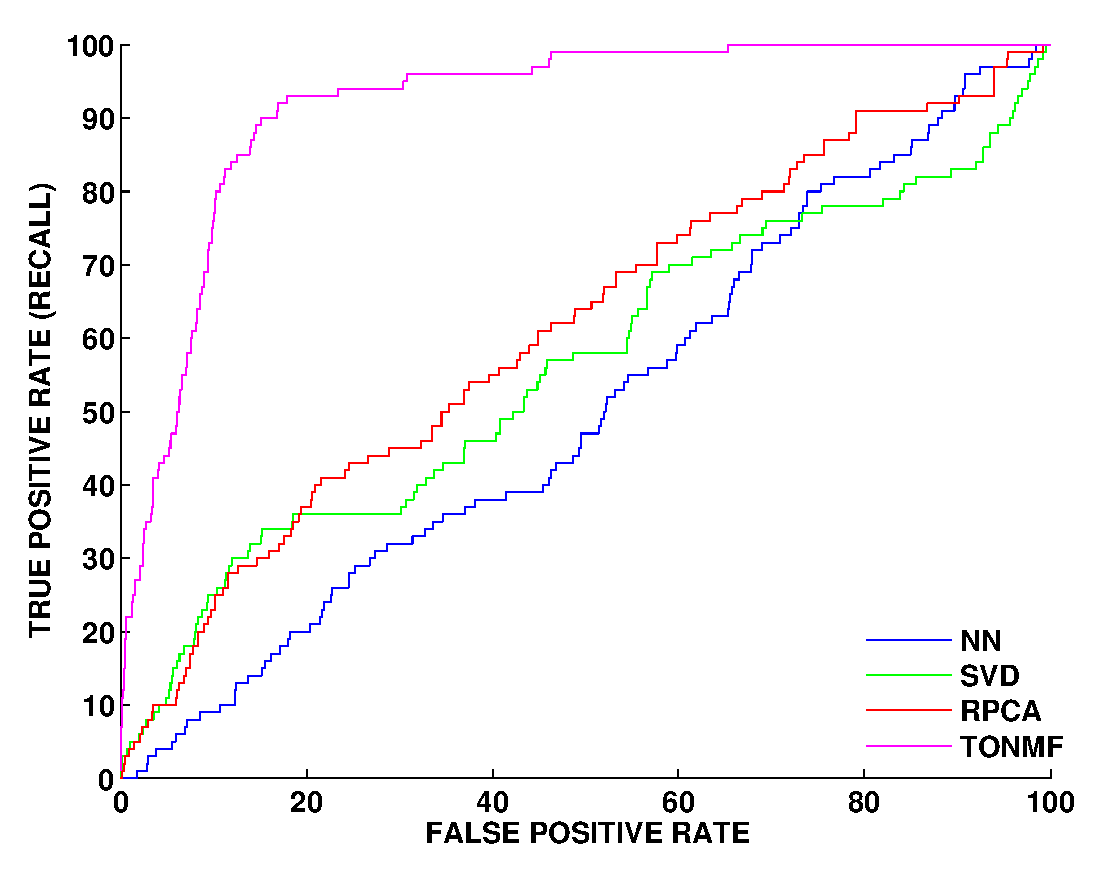
\includegraphics[width=2.4in,height=1.8in]{rocreuters.eps}
  \caption{Reuters}
  \label{fig:rocreuters}
 \end{minipage}%
 \begin{minipage}{0.5\linewidth}
  \centering
  \caption*{Parameter Sensitivity}
  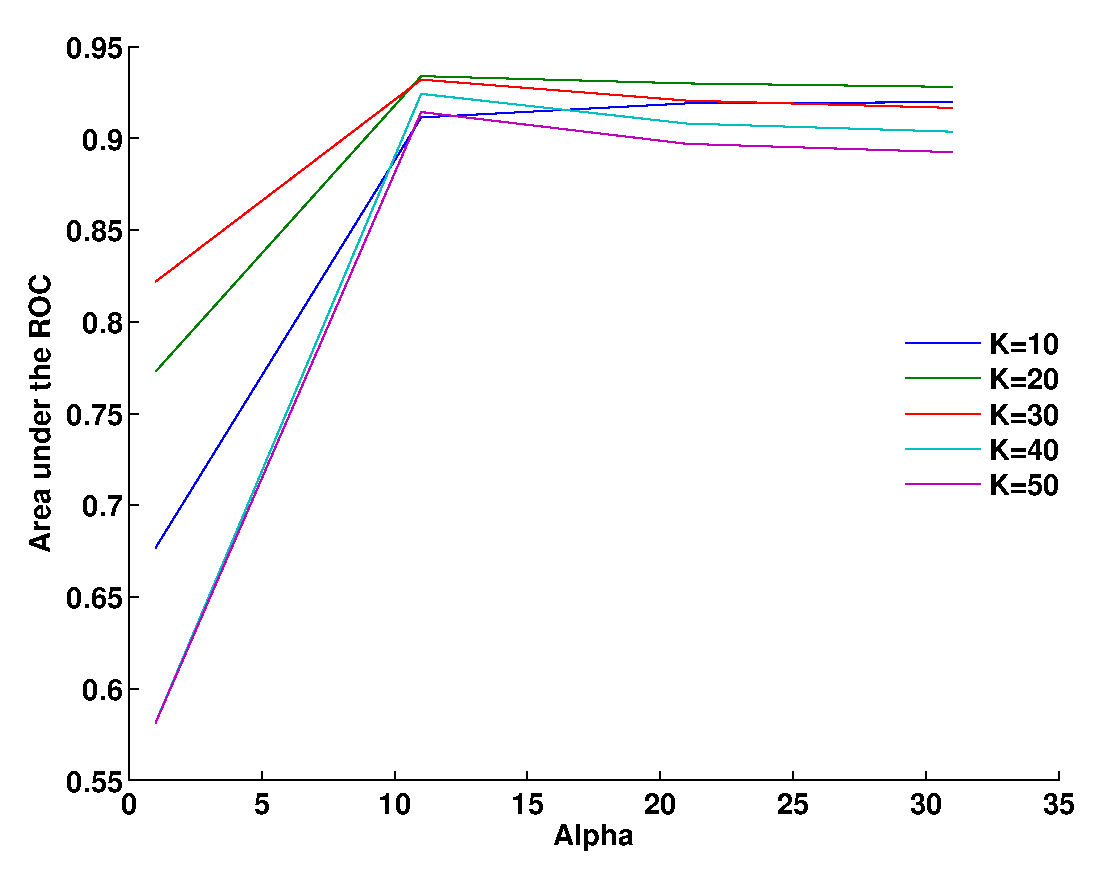
\includegraphics[width=2.4in,height=1.8in]{alphakreuters.eps}
  \caption{Reuters}
  \label{fig:alphakreuters}
 \end{minipage}
 \begin{minipage}{0.5\linewidth}
  \centering
  \caption*{ROC}
  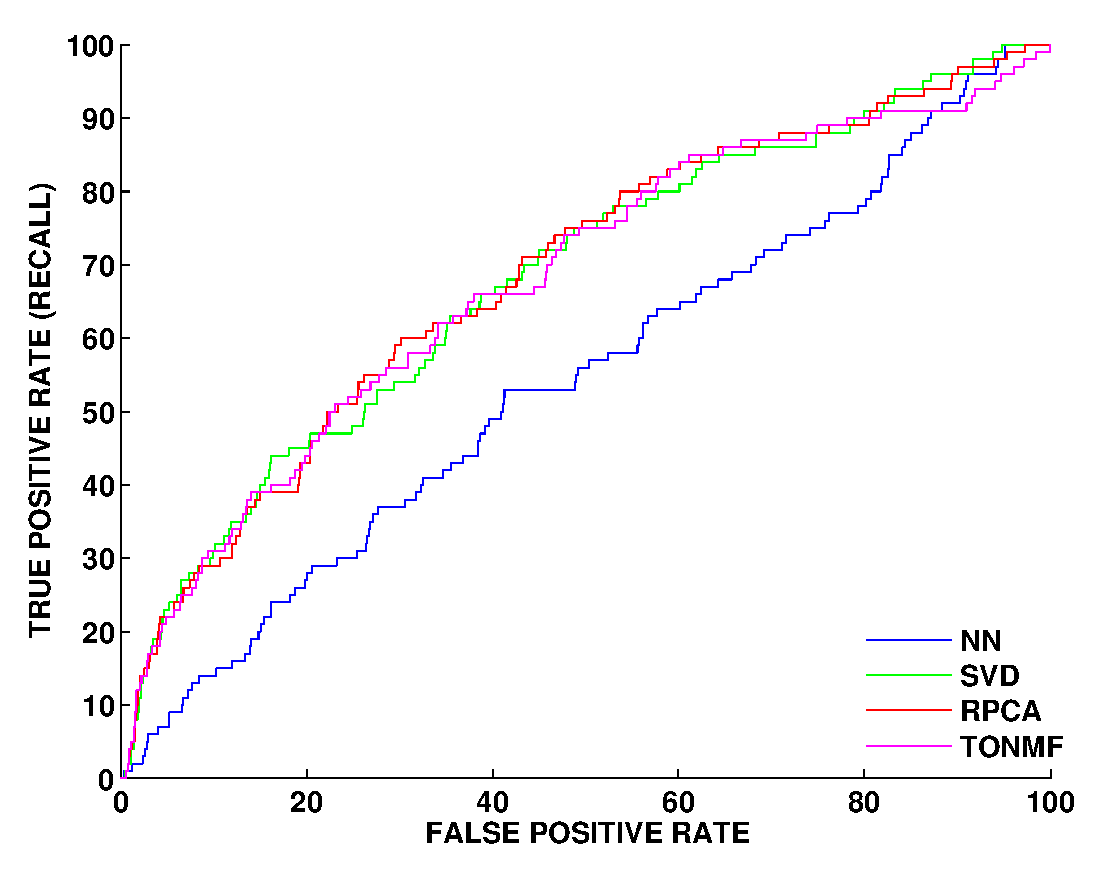
\includegraphics[width=2.4in,height=1.8in]{rocrcv.eps}
  \caption{RCV20}
  \label{fig:rocrcv}
 \end{minipage}%
 \begin{minipage}{0.5\linewidth}
  \centering
  \caption*{Parameter Sensitivity}
  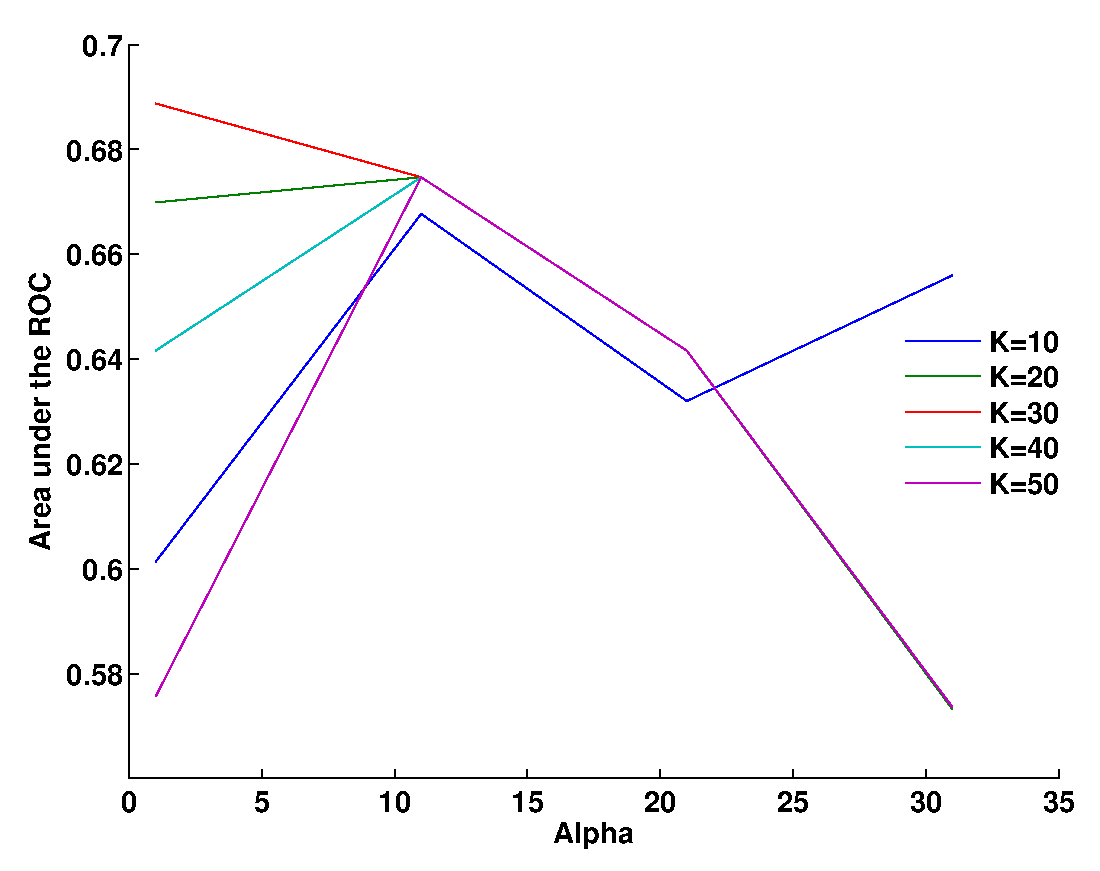
\includegraphics[width=2.4in,height=1.8in]{alphakrcv.eps}
  \caption{RCV20}
  \label{fig:alphakrcv}
 \end{minipage}
  \begin{minipage}{0.5\linewidth}
  \centering
  \caption*{ROC}
  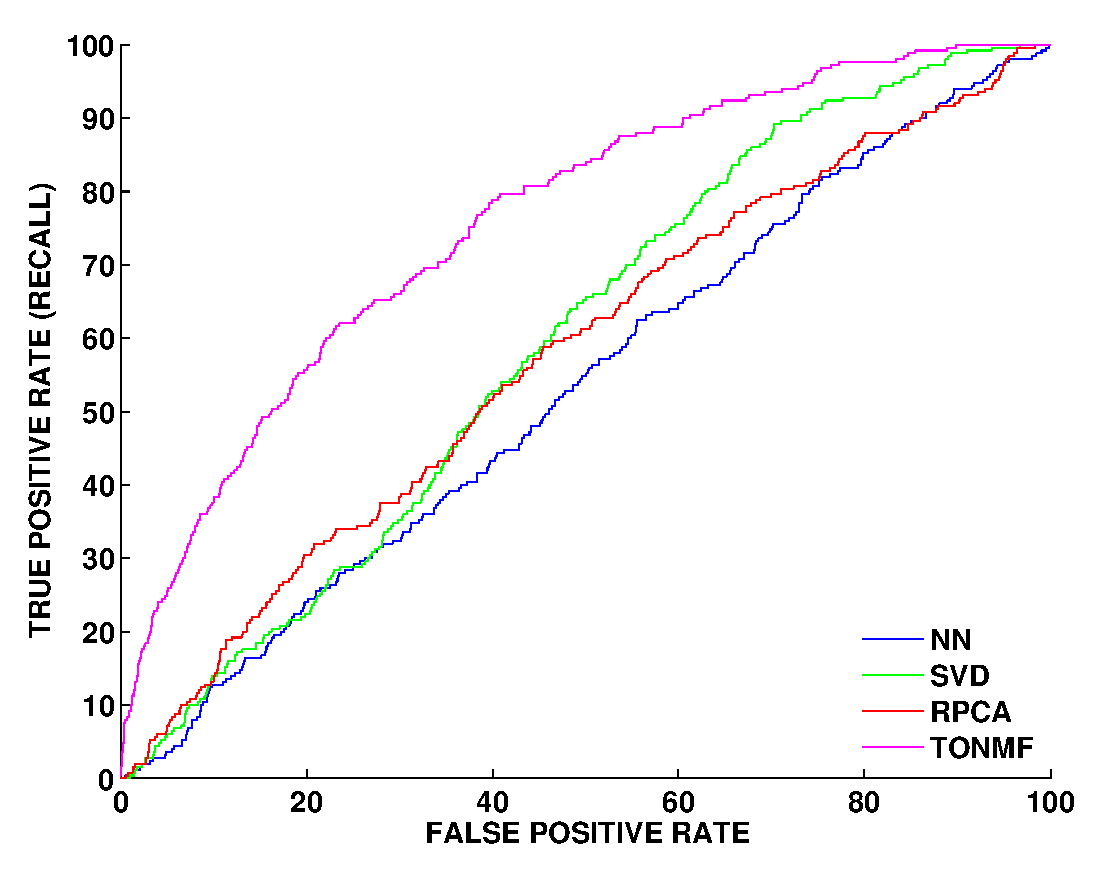
\includegraphics[width=2.4in,height=1.8in]{rocmbsmall.eps}
  \caption{Market Basket}
  \label{fig:rocmb}
 \end{minipage}%
 \begin{minipage}{0.5\linewidth}
  \centering
  \caption*{Parameter Sensitivity}
  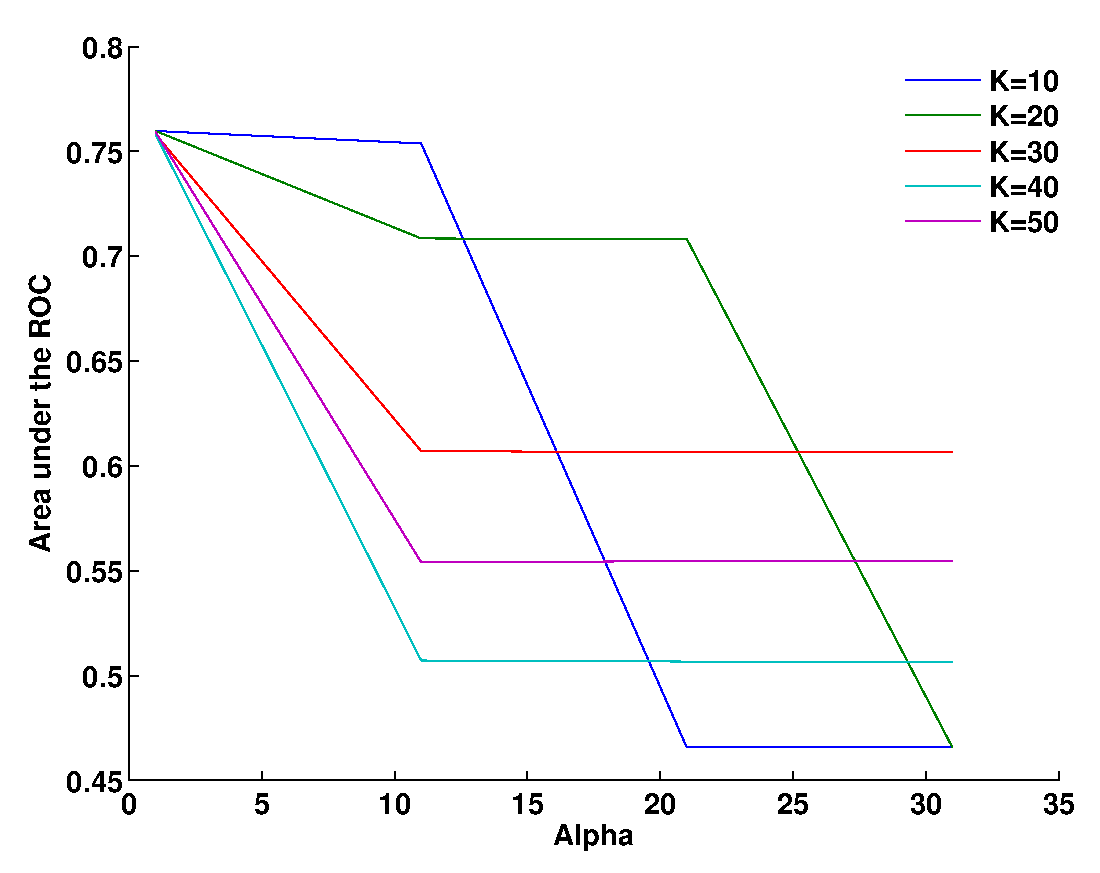
\includegraphics[width=2.4in,height=1.8in]{alphakmbsmall.eps}
  \caption{Market Basket}
  \label{fig:alphakmb}
 \end{minipage}
  \begin{minipage}{0.5\linewidth}
  \centering
  \caption*{ROC}
  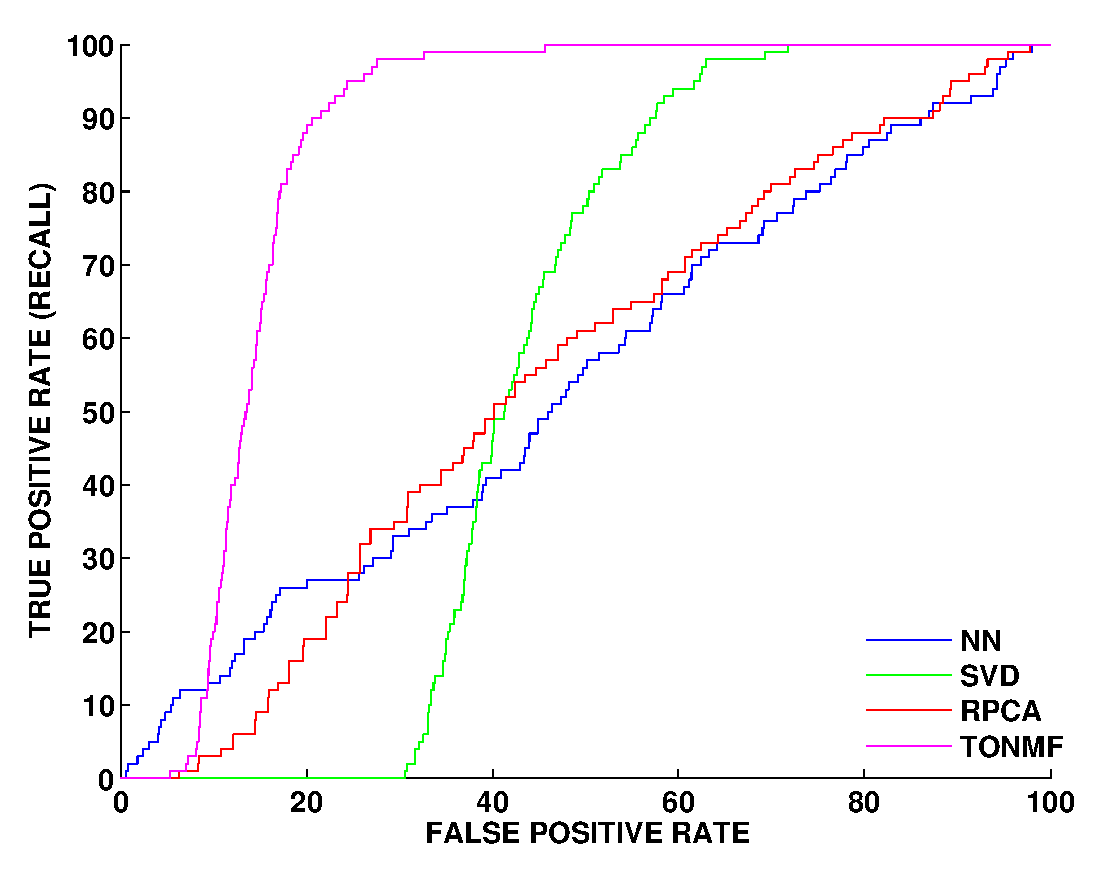
\includegraphics[width=2.4in,height=1.8in]{rocwikippl.eps}
  \caption{Wiki People}
  \label{fig:rocwiki}
 \end{minipage}%
 \begin{minipage}{0.5\linewidth}
  \centering
  \caption*{Parameter Sensitivity}
  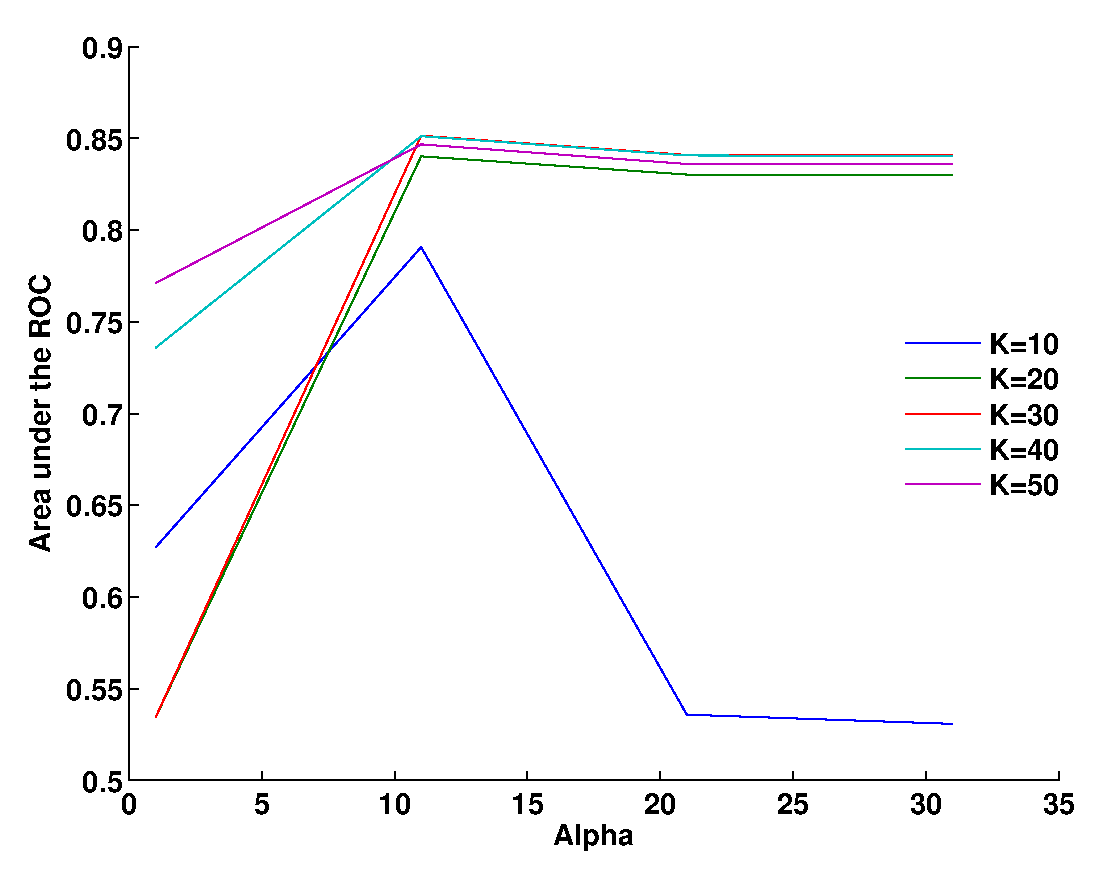
\includegraphics[width=2.4in,height=1.8in]{alphakwikippl.eps}
  \caption{Wiki People}
  \label{fig:alphakwiki}
 \end{minipage}
\end{figure*}

We first present the ROC curves for the different data sets. The ROC
curve for the {\em Reuters} dataset is illustrated in Figure
\ref{fig:rocreuters}. In this case, our algorithm shows a drastic
improvement over both the baseline algorithms.  This is evident from
the rather large lift in the chart.   Our algorithm
\algo\, had an area of 0.9340 under ROC. The $k$-NN approach
performed quite poorly, and had an area under the  ROC curve of
0.5370. This is slightly better than random performance. The area
under ROC for the  $SVD$ method  was  0.5816 and \ramki{$RPCA$ was 0.6120}, which is better than
the $k$-NN method, but still significantly less than the proposed
algorithm.

 The comparison of our algorithm with baselines  for the
{\em RCV20} data set is shown in Figure \ref{fig:rocrcv}. As
discussed in the data generation section, this is a particularly
challenging data set, because of the similarity in the vocabulary
distribution between the rare class, and the regular class. It is
evident that our algorithm \algo\  performed better than the
$SVD$, $RPCA$  and the $k$-NN method. However, the lift in  the ROC curve for
all the methods is not particularly significant, because of the
inherently challenging nature of the data set. The $k$-NN
method performed particularly poorly in this case. In a later
section, we will provide some insights about the fact that some of
this ``poor'' performance is because of the noise in the  data set
itself, where some of the  points in the regular class should really
be considered outliers. We generated a datasets in RCV20 where we just changed the outlier class to {\em christian religion}. We received
a best ROC of 0.9732 and it is not shown in Figure \ref{fig:rocrcv}.

\ramki{ Figure \ref{fig:rocwiki} shows the comparison of our
algorithm $TONMF$ against the baselines for the {\em Wiki People}
data set.  The area under the ROC for $k$-NN was 0.5395, which is
rather poor. All the other methods performed better than $k$-NN with
area under the ROC for $SVD$ being 0.5670 and $RPCA$ being 0.5471.
Our algorithm $TONMF$ performed significantly better than all the
methods with an AUC of 0.8552. Clearly, this is a significant
qualitative difference between the methods. The above three were
experiments on real life dataset and we chose market basket for
synthetic dataset.}

 The ROC comparison for the synthetic  market basket data is illustrated
in Figure \ref{fig:rocmb}. In this case, the improvement of the
algorithm \algo\  over the baseline methods was quite  significant.
Specifically, the algorithm \algo\ had an area under the ROC curve
of 0.7598, which is a significant  lift. This significantly
outperformed the $SVD$ and \ramki{$RPCA$ method, which had an area under the ROC curve
of 0.5731 and 0.5758 respectively}. As in the case of the other data sets, the $k$-NN
algorithm performed very poorly with an area under the ROC curve of
0.5431. The consistently  poor performance of the $k$-NN approach
over all algorithms is quite striking, and suggests that
straightforward generalizations of  outlier analysis techniques from
other data domains are often not well suited to the text domain.

\ramki{Based on our conducted experiments on real world and
synthetic datasets, we observed that $TONMF$ outperformed every
other baseline.  Furthermore, the rank of the methods from  best  to
worst is $TONMF, RPCA, SVD$ and $NN$.} Clearly, conventional
distance-based  methods do not seem to work very well for text data.

\subsection{Parameter Sensitivity}
From (\ref{outlier}) in Section \ref{sec:model}, we can
see that the parameters for our algorithm are $\alpha, \beta$ and
the low rank $r$. We tested the algorithm for different variations
in the parameters,  and found that our algorithm was insensitive to
changes in $\beta$. In other words,  for a given low rank $r$ and
$\alpha$, the changes in the value of  $\beta$ did not result in
significant change in the area under ROC. Hence, in this paper, we
provide the charts of the ROC area  variation with the parameters
$\alpha$ and $r$ on the data sets.

The  sensitivity results for the {\em Reuters} data set are
illustrated in Figure \ref{fig:alphakreuters}. The value of $\alpha$
is illustrated on the $X$-axis, and different values of the low rank
$r$ are graphed by different curves in the plot. It is evident in
this case, that the
 area under the  ROC increased with
increase in low rank $r$ and $\alpha$. However the improvement
started diminishing and changed very marginally at higher ranks $r$.

The results for the {\em RCV20} and \ramki{{\em Wiki People}} datasets are illustrated in Figure \ref{fig:alphakrcv} \ramki{and Figure \ref{fig:alphakwiki} respectively}.
 As in the previous case, the value of $\alpha$ is illustrated on
 the $X$-axis, and  different values of the low rank $r$ are
 represented by different curves. In this case, the area under the
 ROC curve was relatively insensitive  to the parameters. This
 implies that the algorithm can be  used over a wide range of
 parameters, without affecting the performance too much.
Finally, the results for the market basket data set are illustrated
in  Figure \ref{fig:alphakmb}.  In this case, the area under the ROC
curve decreases with increase in low rank $r$ and $\alpha$. This is
because the market-basket data  has inherently very low (implicit)
dimensionality, and  therefore, it is best to use  a relatively low
rank in order to mine the outliers.

\ramki{From the parameter sensitivity graphs for real world
datasets, we observe that for a given $\alpha$, the approach is
relatively insensitive to the rank of the approximation. It needs to
be kept in mind that it is generally faster to determine approximations
with lower rank.  This implies that, for very large matrices, the
algorithm can be made computationally faster by choosing approximations 
with lower rank without compromising on the performance. According to
the model explained in equation \eqref{outlier}, the parameters
$\alpha$ and $\beta$ balance the importance given to outliers
against the  matrix sparsity criterion during regularization. By
picking $\alpha
>> \beta$, the importance of the outlier portion of the regularization
increases. From the parameter sensitivity graph,  it is evident that
for most low ranks $K$, the increase in the value of $\alpha$ does
not improve the performance of the outlier detection. This is
because, beyond a particular limit, the weights given to  the
outlier criterion  do not supersede the optimization problem's main
objective of extracting the low-rank patterns from the underlying
data. }

\subsection{Further Insights} \label{sec:insights}
In order to illustrate the inner workings of  the matrix
factorization approach, we provide some further insights about the
statistics buried deep in the algorithm. We also present some interesting
observations when outliers share the same vocabulary distribution as
regular data points, as is the case for the {\em RCV20} data set.
One observation is that the method of data generation implicitly
assumes that all the documents within a ``regular'' class in a real
data set are not outliers. This is of course not true in practice,
since some of the documents within these classes will also be
outliers, for reasons other than topical affinity.  Our algorithm
\algo\ was also able to  detect such distinct documents, much better
than the other baseline algorithms. We isolated those false
positives of our algorithm \algo\ that were not detected in the
baselines in the case of the {\em RCV20} data set. It was observed
that while these outliers officially belonged to one of the regular
classes, they did show different {\em kinds} of distinctive
characteristics. For example, while the average number of words in
regular documents was 195, the ``false positive'' outliers chosen by
our algorithm were typically either very lengthy with  over 400
words, or were unusually short will less than 150 words.  This
behaviour was also generally reflected in the number of distinct
words per document. Another observation is that these outlier
documents typically had a significant vocabulary repetition over a
small number of distinct words. Thus,  the algorithm was also able
to identify those natural outliers, which {\em ought to} have been
considered outliers for reasons of statistical word distribution, as
opposed to their topical behaviour.

% \begin{figure}[ht]
% \centering
% \subfigure[Neutral Smiley]{%
 % \includegraphics[width=3.2in,height=2in]{rocmbsmallcomp.eps}.
% \label{fig:subfigure1}}
% \quad
% \subfigure[Blush Smiley]{%
% 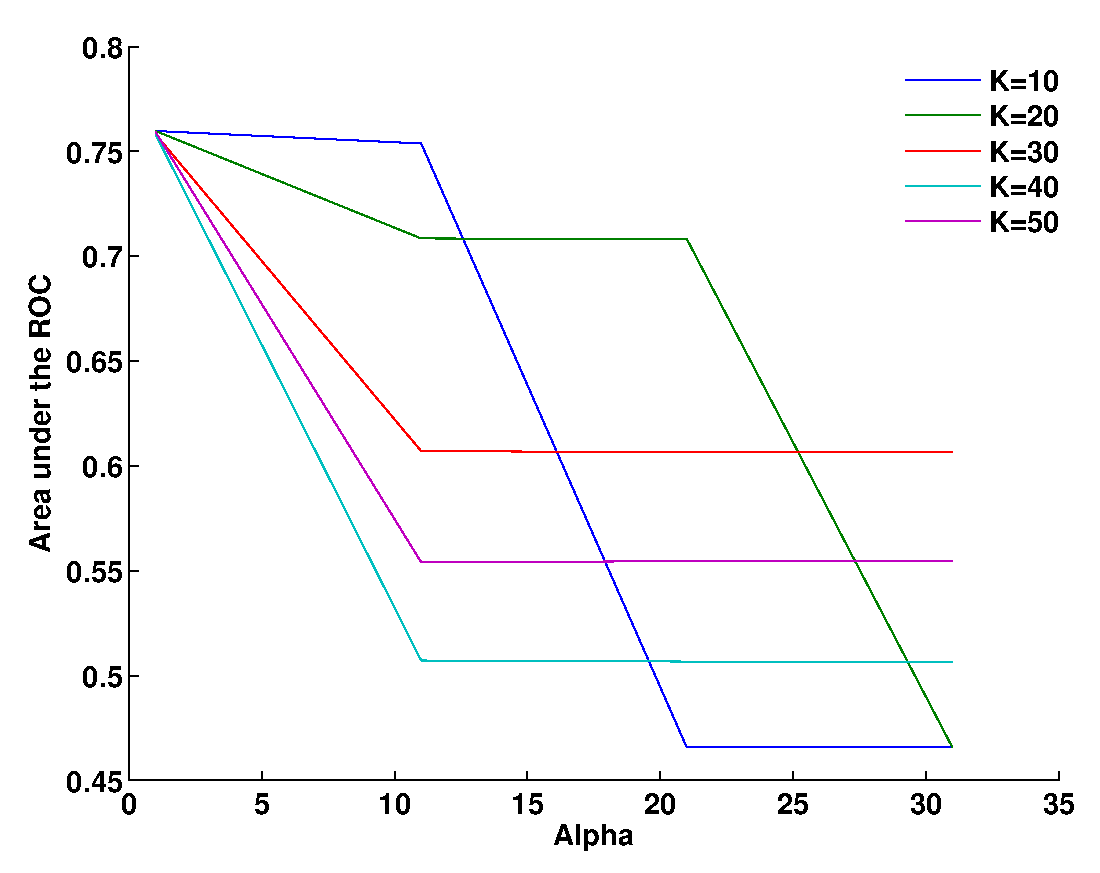
\includegraphics[width=3.2in,height=2in]{alphakmbsmall.eps}
% \label{fig:subfigure2}}
% \subfigure[Sleepy Smiley]{%
% 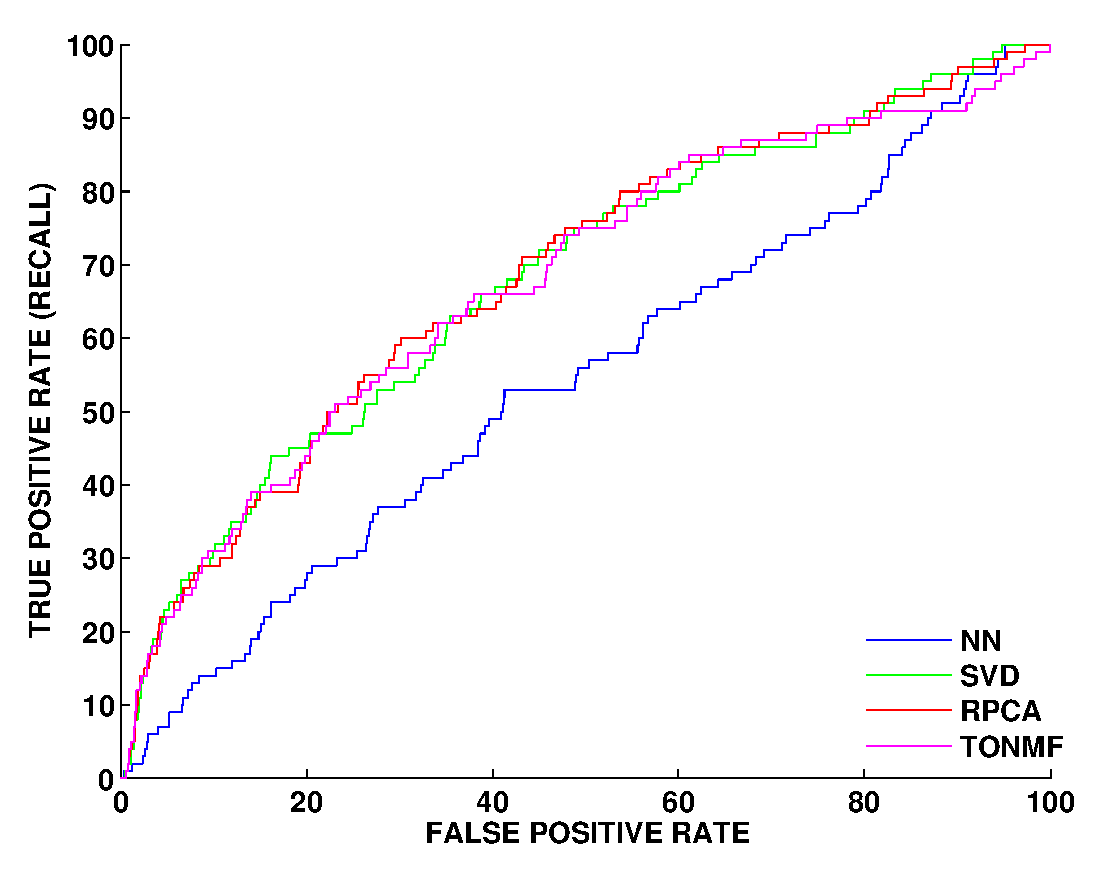
\includegraphics[width=3.2in,height=2in]{rocrcv.eps} .
% \label{fig:subfigure3}}
% \quad
% \subfigure[Angry Smiley]{%
% 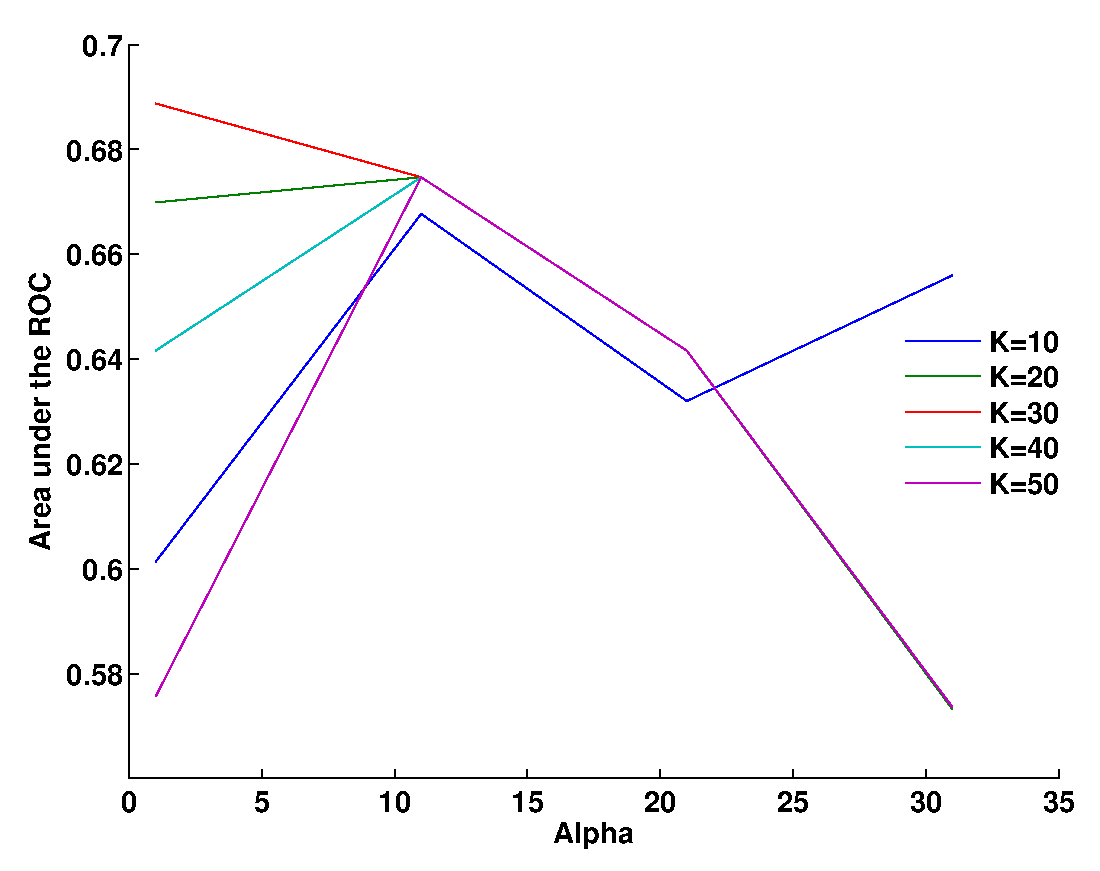
\includegraphics[width=3.2in,height=2in]{alphakrcv.eps}
% \label{fig:subfigure4}}
% \subfigure[c]{
% 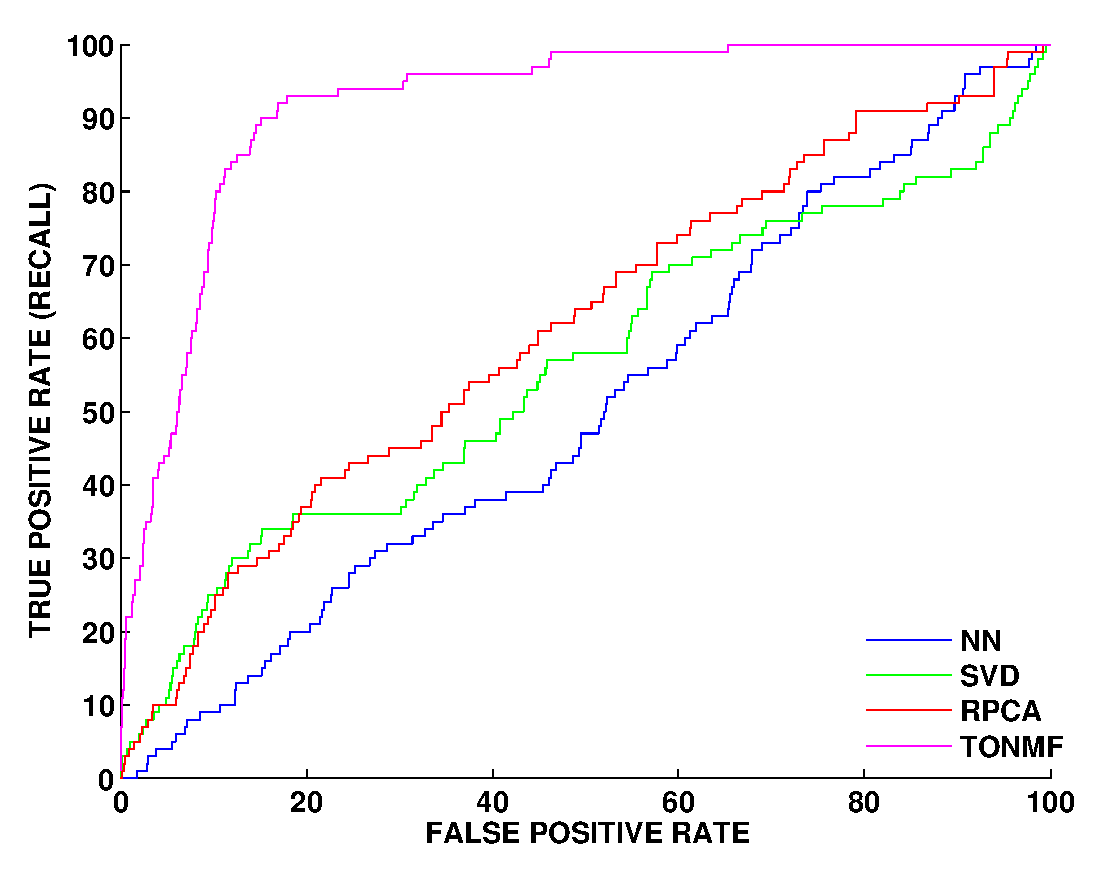
\includegraphics[width=3.2in,height=2in]{rocreuters.eps}
% \label{c}}
% \quad
% \subfigure[d]{
% 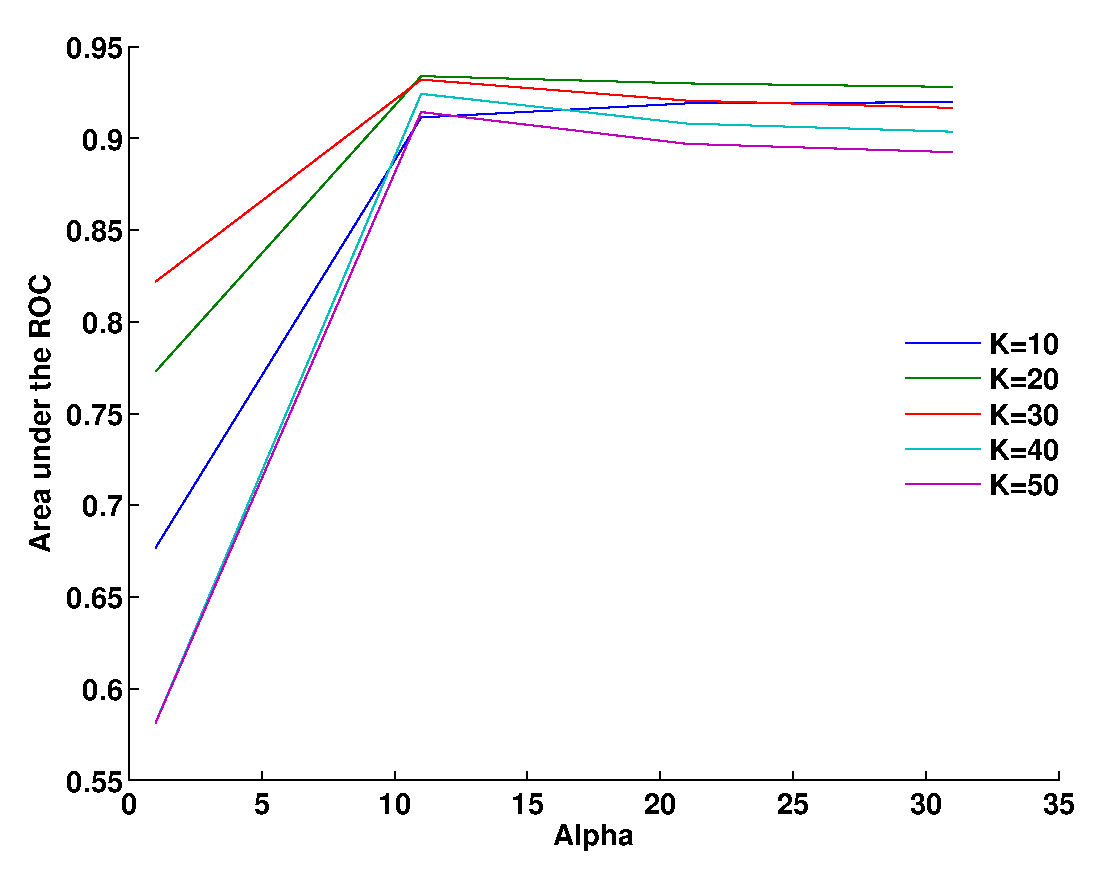
\includegraphics[width=3.2in,height=2in]{alphakreuters.eps}
% \label{d}}
% \caption{Main figure caption}
% \label{fig:figure}
% \end{figure}
